\documentclass{bioinfo}
%\usepackage{amsmath}
%\usepackage{enumerate}
\usepackage{graphicx}
%\author{R.Y.~Neches \& E.G.~Wilbanks} 
%\title{Analyzing ChIP-seq data with Pique}

%\addtolength{\oddsidemargin}{-.875in}
%\addtolength{\evensidemargin}{-.875in}
%\addtolength{\textwidth}{1.75in}
%\addtolength{\topmargin}{-.875in}
%\addtolength{\textheight}{1.75in}

\copyrightyear{2011}
\pubyear{2011}

% This writeup is intended to be submitted to Bioinformatics as an
% Applicaiton Note under either the Gene Expression or Sequence
% Analysis. These are the instructions to authors :
%
% Application Notes (up to 2 pages; this is approx. 1300 words or 1000
% words plus one figure) : Applications Notes are short descriptions
% of novel software or new algorithm implementations, databases and
% network services (web servers, and interfaces). Software or data
% must be freely available to non-commercial users. Availability and
% Implementation must be clearly stated in the article. Authors must
% also ensure that the software is available for a full TWO YEARS
% following publication. Web services must not require mandatory
% registration by the user. Additional Supplementary data can be
% published online-only by the journal. This supplementary material
% should be referred to in the abstract of the Application Note. If
% describing software, the software should run under nearly all
% conditions on a wide range of machines. Web servers should not be
% browser specific. Application Notes must not describe trivial
% utilities, nor involve significant investment of time for the user
% to install.
%
% Software : If the manuscript describes new software tools or the
% implementation of novel algorithms the software must be freely
% available to non-commercial users at the time of submission, and
% appropriate test data should be made available. Availability must be
% clearly stated in the article. Authors must also ensure that the
% software and test data is available for a full TWO YEARS following
% publication. The editors of Bioinformatics encourage authors to make
% their source code available and, if possible, to provide access
% through an open source license (see www.opensource.org for
% examples). Authors should make every effort to use URLs that will
% remain stable. At the minimum, authors must provide one of:
% webserver, source code or binary.
%
% http://www.oxfordjournals.org/our_journals/bioinformatics/

\begin{document}
\firstpage{1}

\title[In a fit of pique]{Analyzing microbial ChIP-Seq data with
  Pique} \author[Neches
\textit{et~al}]{R.Y.~Neches\,$^{1,3}$\footnote{to whom correspondence
    should be addressed}, E.G.~Wilbanks\,$^{1,3}$ and
  M.T.~Facciotti\,$^{2,3}$
  \address{$^{1}$Microbiology Graduate Group, University of California, Davis.\\
    $^{2}$Department of Biomedical Engineering, University of
    California, Davis.\\$^{3}$Genome Center, University of California,
    Davis.}}

\history{Received on XXXXX; revised on XXXXX; accepted on XXXXX}

\editor{Associate Editor: XXXXXXX}

\maketitle

\newcommand{\imsize}{1.0\columnwidth}
%\newcommand{\threeup}{0.26\columnwidth}
%\newcommand{\cotwo}{$\text{CO}_{2}$}
%\newcommand{\htwo}{$\text{H}_2$}
%\newcommand{\otwo}{$\text{O}_2$}
%\newcommand{\water}{$\text{H}_2\text{O}$}
%\newcommand{\htwos}{$\text{H}_2\text{S}$}

\begin{abstract}
\section{Motivation:}

\noindent While numerous effective peak finders have been developed
for eukaryotic systems, we have found that the approaches used can be
suprisingly error prone when run on high-coverage bacterial and
archaeal ChIP-Seq datasets.

% Why not? Examples, evidence, hypothesis. 

\section{Results:}

\noindent We have developed Pique, a conceptually simple, easy to use
ChIP-Seq peak finding application for bacterial and archaeal ChIP-Seq
data. The software is cross-platform and Open Source, and based on
Open Source dependencies. Output is provided in standardized
bioinformatic formats, and easily imported by the Gaggle Genome
Browser for manual curation and data exploration, or into statistical
computing and graphics software such as R for further analysis.

\section{Availability:} 

\noindent The software is available under the BSD-3 license at

\href{http://github.com/ryneches/pique}{http://github.com/ryneches/pique}.

\noindent A tutorial and test data are included with the documentation.

\section{Contact:} \href{ryneches@ucdavis.edu}{ryneches@ucdavis.edu}

\end{abstract}

\section{Introduction}

\noindent Next generation sequencing coupled with chromatin
immuno\-pre\-cipi\-tation (ChIP-Seq) is revolutionizing our ability to
genomically map protein-DNA associations for a wide variety of
proteins.  The growing popularity of ChIP-Seq has spurred the
development of over thirty peak picking algorithms (for a nearly
completely list see \cite{wilbanks}). The relative performance of
representative peak detection algorithms on eukaryotic data and
methods to assess performance have been recently reviewed by several
authors \cite{Pepke, Laajala_review, too_many_peak_callers,
  peakranger, peak_benchmark}.

While ChIP-Seq has been predominantly used to interrogate protein-DNA
interactions in eukaryotic systems, there are clear advantages to
adopting this technology for studying microbes. Microbial genomes are
typically smaller than eukaryotic genomes (the genome of {\em E. coli}
is about 2000 times smaller than that of humans), and have simpler
replicon and chromatin structure.

Only one ChIP-Seq analysis tool, CSDeconv \cite{CSDeconv}, has been
explicitly developed for microbial data. This MATLAB package
successfully finds peaks in microbial ChIP-Seq data, but its
application is limited by its dependency on costly proprietary
software, slow performance, lack of support for manual
curation. Herein we describe Pique, a conceptually simple,
Python-based peak finding package that enables easy and rapid peak
finding in bacterial and archaeal ChIP-Seq datasets.

\section{Approach}

\noindent ChIP-Seq in bacteria and archaea yields coverage several
orders of magnitude larger than in eukaryotic systems, resulting in
continuous coverage rather than the sparse coverage typically present
in eukaryotic ChIP-Seq data.  This feature of microbial ChIP-Seq
experiments permits simpler, faster algorithms to be used. We have
based our algorithm on classic noise reduction techniques from signal
processing.

Pique is designed for use in systems that have genomic complexities
such as IS elements, gene dosage polymorphisms and accessory genomes
that cause coverage variations unrelated to ChIP, or in cases where
the organism under study is not identical to the reference genome. The
resulting enrichment ``pedestals'' and ``holes'' can be problematic
for detecting peaks and calculating enrichment levels. If the user
provides a map of these features, the software will automatically
perform a segmented analysis.

The wide variety of microbial systems, target proteins, protocols, and
experimental conditions, calls for fairly tailored statistical
approaches to ChIP-Seq. Instead of attempting to anticipate each of
these (and their combinations) by presenting the user with a very
large number of statistical and heuristic parameters, we have chosen
to focus on the aspects of the analysis that are in common; finding
putative peaks and estimating binding coordinates and binding
affinities. The determination of statistical significance is usually
quite easy for any particular experiment, but is quite difficult to
accurately generalize.

We address this in two ways. First, we provide a quantities for each
peak that can be used to ascertain which peaks are statistically
significant (usually, this involves little more than sorting the table
and choosing a cutoff). Second, we provide integrated support for
curation using the Gaggle Genome Browser. This permits interactive
curation of the peak list and analysis of the ChIP-Seq data in the
context of other Gaggle-enabled resources. Interactive curation of a
microbial ChIP-Seq data set can typically be completed in a few
minutes.

\begin{methods}
\section{Methods}

\noindent Pique requires BAM files as input\cite{sam_format}.
Therefore, prior to using Pique, Illumina (Solexa) reads should first
be quality filtered, quality trimmed, and aligned to a reference
genome, preferably using all contigs of the reference genome as the
mapping target. 

By default, Pique treats each contig as a single analysis region, but
the user may optionally designate regions within a contig for separate
analysis by supplying a feature map.  This may be useful when coverage
levels are systematically altered over large regions.  Pique supports
three features types; analysis regions, masking regions, and
normalization regions. Masking regions are simply masked out of their
respective analysis regions, and are useful for removing coverage
variation due to repetitive DNA. Normalization regions selected within
an analysis region, are used to compensate for total coverage
discrepancies between the background and ChIP alignments.

The user launches the primary analysis stage by providing alignment an
file for the ChIP data, an alignment file for the control data, and
optional an coverage feature map. The primary analysis proceeds thusly
:

\begin{itemize}

\item The alignment files are digested into coverage tracks, and the
  analysis regions are initialized in memory. Provided masking regions
  are applied.

\item The coverage noise threshold is measured by comparing the
  relative total coverage within the normalization regions. (The user
  should choose normalization regions that contain neither peaks nor
  coverage level aberrations.)

% This no longer happens in the current version, as of August 18, 2011
%
%\item In each analysis region, the ``DC'' component is removed using
%  linear detrending. This removes effects due to coverage variation
%  features larger than about 100Kb.

\item High-$k$ noise in coverage is removed using a Wiener-Kolmogorov
  filter. The filter delay $\alpha$ is chosen to approximate to the
  expected footprint size of the targeted protein. The choice of
  filter implies the existence of two inputs; a ``true'' signal, and a
  noise source. Both are assumed to be stationary stochastic processes
  combined additively.

  % The Wiener-Kolmogorov filter was the first and simplest
  % statistical signal filter, first published by Norbert Wiener in
  % 1949, and independently derived in discrete-time form by Andrey
  % Kolmogorov in 1941.

\item A Blackman window of a diameter equal to the read length is
  convolved with the filtered coverage track to remove features
  smaller than one read. 

\item The noise threshold in the ChIP coverage track is measured by
  comparing the coverage distribution in the ChIP track to the control
  track within user-annotated non-peak regions. Features that exceed
  the noise threshold are identified.

\item The coverage enrichment is distributed differently between the
  forward and reverse strands because the possible read orientations
  are constrained by the fragment size. Pique exploits this by
  requiring that the stop coordinate of the forward strand enrichment
  envelope must fall between the coordinates of the reverse strand
  enrichment envelope, and that the start coordinate of the reverse
  strand enrichment envelope fall between the coordinates of the
  forward strand enrichment envelope. (We call this the overlap
  criterion.)

\end{itemize}

% FIXME : The overlap criterion is a very crude version of the
% heuristic models other peak callers user. We should say something
% here about these models, and why decided not to use them.

\noindent For each putative peak, Pique calculates the enrichment
ratio of the ChIP alignment to the control alignment, the binding
coordinate, and the enrichment normalization factor for that analysis
region. 

\end{methods}

% \begin{figure}[!tfbd peak - a nice one]%figure1
%   % \centerline{\includegraphics{example_data.png}
%   \begin{center}
%     {\resizebox{\imsize}{!}{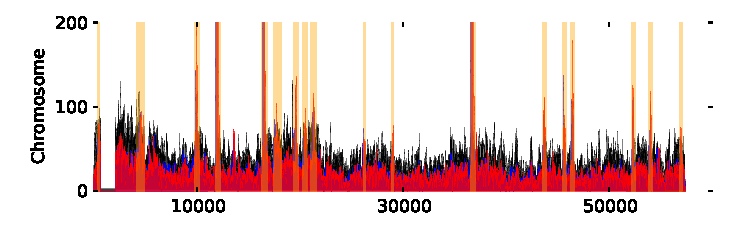
\includegraphics{chr_example.pdf}}}
%     %{\resizebox{\imsize}{!}{\includegraphics{../PNRC200_0:21851.pdf}}}
%     %{\resizebox{\imsize}{!}{\includegraphics{../PNRC200_47121:88549.pdf}}}
%   \end{center}
%   \caption{Peaks found in the chromosome of the included sample
%     dataset, derived from ChIP-seq of tfbD in {\em Halobacterium
%       salinarum} sp. NRC1. Blue and red indicate coverage of reads
%     aligned from the ChIP-derived data to the forward and reverse
%     strands of the genome, respectively. Black indicates coverage
%     aligned from the whole cell extract data. Orange indicates a
%     detected peak. The maximum coverage in this data is 3204, but is
%     shown here truncated at 200.}\label{fig:01}
% \end{figure}

\begin{figure}[!tfbd data - reasonable spot showing curation]%figure2
  \begin{center}
    {\resizebox{\imsize}{!}{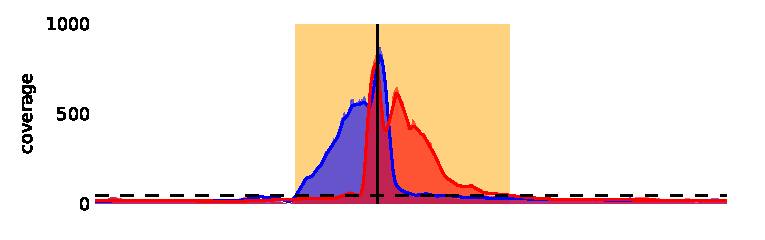
\includegraphics{peak_example.pdf}}}
    {\resizebox{\imsize}{!}{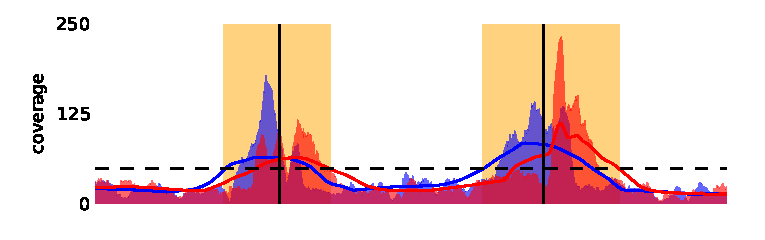
\includegraphics{peak_example_2.pdf}}}
  \end{center}
  \caption{Peaks found in the included sample dataset, derived from
    ChIP-seq of tfbD in {\em Halobacterium salinarum} sp. NRC1. Blue
    and red shading indicate coverage of reads aligned from the
    ChIP-derived data to the forward and reverse strands,
    respectively. Blue and red lines represent the filtered coverage
    levels for the forward and reverse strands, respectively. The
    dashed line is the detected noise threshold for the region. Orange
    indicates a detected peak.}\label{fig:02}
\end{figure}

\section{Discussion}

Pique does not attempt to filter peaks that are statistically
insignificant. We have found that this part of the analysis is rather
specific to the data and to the experiment. Pique is designed to
achieve a low false-negative rate, which comes at the cost of a
relatively high false-positive rate. Thus, some kind of post-filtering
is necessary. Pique provides the user with output that can be used to
support a variety of such statistical tests.

Some recommended filtering might include eliminating peaks that are
significantly narrower than the size range of the sequencing library,
peaks with a normalized enrichment ratio below unity, or peaks that
have predicted binding sites that are very skewed from the center of
the enriched region. Depending on how many peaks are recovered, the
user may wish to try one or all of these, perhaps with
clustering. However, if a ``perfect'' peak list is required, we do not
recommend relying on statiastical refinements alone. To facilitate
manual curation, Pique outputs a track file of the coverage, a
quantitative positional data of the estimated binding sites, and a
bookmark file annotating the peaks. These files are simple to process
by a variety of tools, and can be loaded directly into the Gaggle
Genome Browser.\footnote{See supplementary figure.}

\section{Conclusion}

We conclude that Pique provides a rapid, open source platform for the
sensitive detection of transcription factor binding sites in bacterial
and archaeal ChIP-seq experiments. We leverage standard signal
processing algorithms to rapidly identify binding sites. Downstream
analysis is supported via integration with statistical and graphics
software such as R, and curation via integration with the
user-friendly Gaggle Genome Browser and the suite of Gaggle tools.

We note that Pique should also work well with eukaryotic datasets
provided they are gathered with greater coverage than has been
previously reported.

\section*{Acknowledgement}
\paragraph{Funding\textcolon} 

This project was funded by UC Davis startup funds to M.T.F., NSF Graduate
Research Fellowship awarded to E.G.W. and DARPA award number
HR0011-05-1-0057 to R.Y.N.

%\bibliographystyle{natbib}
%\bibliographystyle{achemnat}
%\bibliographystyle{plainnat}
%\bibliographystyle{abbrv}
%\bibliographystyle{bioinformatics}

\bibliographystyle{plain}

\bibliography{writeup}

\end{document}